\documentclass[11pt]{article}
\usepackage[T1]{fontenc}
\usepackage[margin=0.80in]{geometry}
\usepackage{amsmath,amssymb,amsthm}
\usepackage{graphicx}
\usepackage{booktabs,tabularx}
\usepackage[hidelinks]{hyperref}
\usepackage{microtype}

\newtheorem*{theorem}{Endpoint counterexample}
\newcommand{\Ent}{\operatorname{Ent}}
\newcommand{\E}{\mathcal E}
\newcommand{\XiN}{\Xi^{(n)}}

\title{A singular endpoint in the R\'enyi--Sobolev asymptotic-tightness theorem}
\author{Counterexample/correction for arXiv:2306.12288}
\date{13 August 2026}

\begin{document}
\maketitle

\section*{Proof intuition}
Order-zero entropy measures only how much of the space is in the support.
To make it positive, a function must have a hard zero.  For $q>1$, the
factor $f^{q-1}$ also vanishes at that zero, so the edge energy stays finite.
Exactly at $q=1$, the factor turns into $\ln f$ and a hard zero becomes an
infinite barrier.  Below one it becomes a negative power and is singular
again.  The endpoint is therefore a genuine phase transition hidden by the
notation ``$q\ge1$''.

\begin{theorem}
For the binary Bonami--Beckner semigroup and every $n\ge1$,
\[
  \XiN_{0,1}(\alpha)=+\infty
  \qquad(0<\alpha<\ln2).
\]
Thus Theorem~2 of the source is false at the explicitly included endpoint
$(p,q)=(0,1)$: it claims convergence to the finite number
\[
 \Xi_1(\alpha)=\left(\frac12-y\right)
       \ln\frac{1-y}{y},\qquad
 y=h^{-1}(\ln2-\alpha)\in(0,\tfrac12).
\]
The theorem's lower bound remains true; its claimed asymptotic tightness at
this endpoint does not.
\end{theorem}

\section*{The exact claim in the source}
Theorem~2 says ``for $p\ge0,q\ge1$'' and therefore includes $p=0,q=1$.
Its binary specialization again asserts asymptotic tightness throughout
$p\ge0,q\ge1$ and $0\le\alpha<\ln2$.  The source's own formula~(17) gives
the finite value of $\Xi_1$ displayed above.

\begin{center}
\begin{minipage}[t]{0.48\textwidth}
\centering
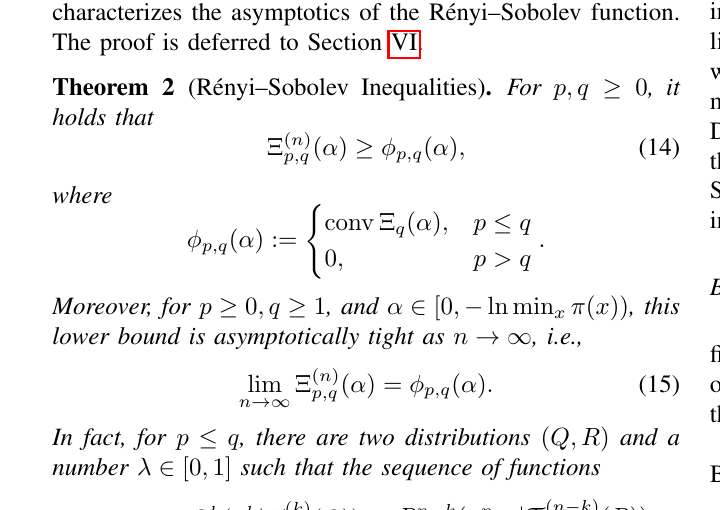
\includegraphics[width=\linewidth]{evidence/theorem_endpoint_crop.png}

{\scriptsize Theorem~2, official arXiv PDF page 4.}
\end{minipage}\hfill
\begin{minipage}[t]{0.48\textwidth}
\centering
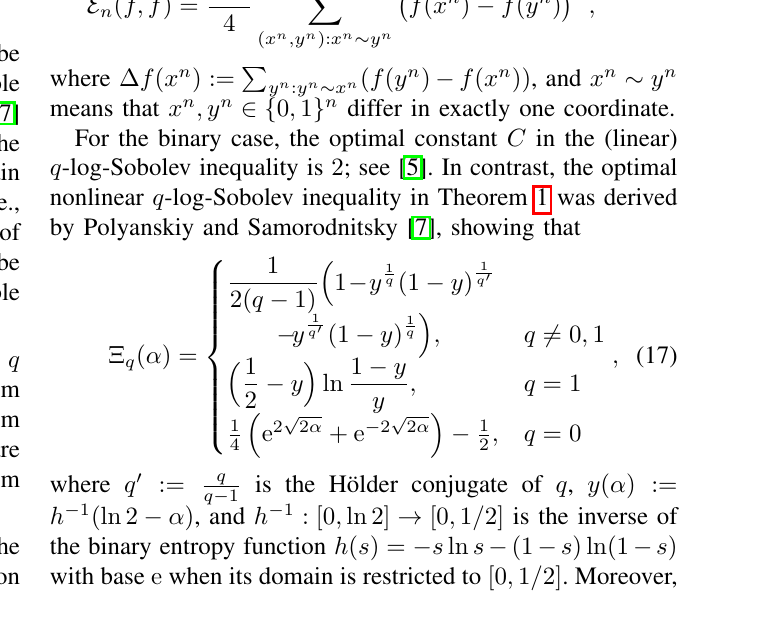
\includegraphics[width=\linewidth]{evidence/binary_formula_crop.png}

{\scriptsize Finite binary formula~(17), official PDF page 4.}
\end{minipage}
\end{center}

\clearpage
\section*{Proof of the counterexample}
Write $Q_n=\{0,1\}^n$ and let $\pi^n$ be uniform measure.  The source defines
the order-zero two-parameter entropy of every nonnegative function by
\[
 \Ent_{0,q}(f)=-\ln\pi^n(f>0).
\]
Let $f$ be nonzero and satisfy
$n^{-1}\Ent_{0,1}(f)\ge\alpha>0$.  If
$S=\{x:f(x)>0\}$, then
\[
  \ln\frac{2^n}{|S|}\ge n\alpha>0.
\]
Hence $S$ is nonempty and proper.  Since the hypercube is connected, an
edge $x\sim y$ crosses its boundary.  Relabel it so that
$f(x)=a>0$ and $f(y)=0$.

At $q=1$ the source uses the continuous endpoint
\[
 \frac1n\,\frac{\E_n(f,\ln f)}{\mathbb E_{\pi^n}f}.
\]
To evaluate it at a function with zeros, replace every zero of $f$ by
$\varepsilon>0$.  The symmetrized edge formula for the Dirichlet form
contains, on the selected boundary edge, a fixed positive multiple of
\[
 (a-\varepsilon)(\ln a-\ln\varepsilon).
\]
All edge summands are nonnegative because the logarithm is increasing.
The displayed term tends to $+\infty$ as $\varepsilon\downarrow0$, whereas
$\mathbb E f_\varepsilon\to\mathbb E f>0$.  Therefore the endpoint energy
of every feasible $f$ is $+\infty$.

This proves $\XiN_{0,1}(\alpha)=+\infty$.  The constraint is not vacuous:
a singleton support has entropy $n\ln2$, so it is feasible for every
$\alpha<\ln2$.  If instead one interprets the $q=1$ endpoint as admitting
only strictly positive $f$, the conclusion is identical by the standard
extended-real convention: every such $f$ has $\Ent_{0,1}(f)=0$, so the
positive-$\alpha$ feasible class is empty and its infimum is $+\infty$.

For comparison, when $0<\alpha<\ln2$ the source formula has
$0<y<1/2$, hence
$(1/2-y)\ln((1-y)/y)$ is a finite positive real number.  An identically
infinite sequence cannot converge to it.

\section*{One-bit calculation}
The singularity is already visible before taking products.  For
$f_\varepsilon=(1,\varepsilon)$, the source's one-bit generator gives
\[
 \frac{\E(f_\varepsilon,\ln f_\varepsilon)}{\mathbb E f_\varepsilon}
 =\frac{1-\varepsilon}{2(1+\varepsilon)}
    \ln\frac1\varepsilon \longrightarrow+\infty.
\]
This is the complete obstruction in its smallest form.

\clearpage
\section*{Where the proof fails}
The asymptotic-tightness proof reduces to $p=0$ and conditions a product
distribution on a typical set.  That distribution has zeros.  Fact~1 then
asserts a uniform energy bound for every distribution and every $q\ge1$,
on the ground that the expression is continuous on the closed probability
simplex.  At $q=1$ this is false.

\begin{center}
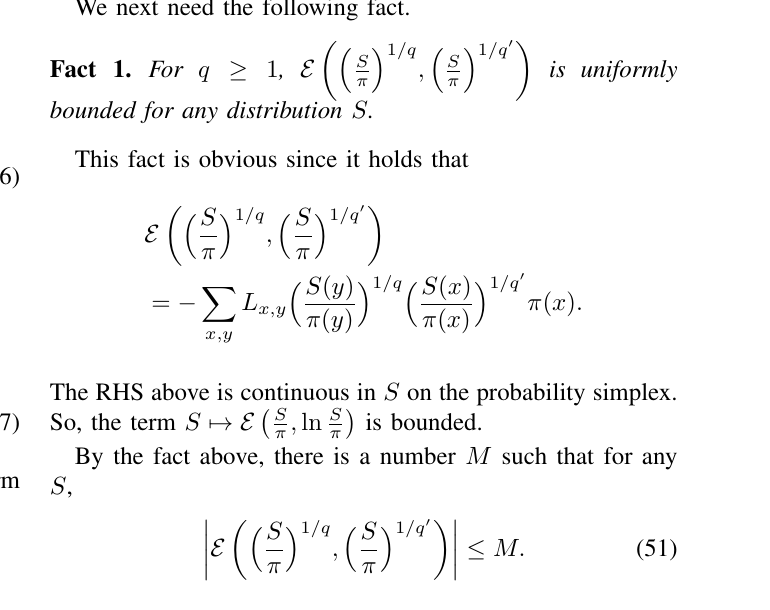
\includegraphics[width=0.82\textwidth]{evidence/proof_fact_crop.png}

{\scriptsize Fact~1 and its continuity claim, official arXiv PDF page 11.}
\end{center}

Indeed, on the binary space take
$S_\varepsilon=(1-\varepsilon,\varepsilon)$.  Since
$\pi=(1/2,1/2)$, direct substitution gives
\[
 \E\!\left(\frac{S_\varepsilon}{\pi},
              \ln\frac{S_\varepsilon}{\pi}\right)
 =\frac12(1-2\varepsilon)
       \ln\frac{1-\varepsilon}{\varepsilon}
 \longrightarrow+\infty.
\]
Consequently the constant $M$ invoked immediately after Fact~1 does not
exist at $q=1$.

Nor can the construction be repaired by smoothing the typical-set law.
Adding any positive background multiple of $\pi^n$ makes the law have full
support, and its order-zero R\'enyi divergence becomes exactly zero; it then
fails every constraint with $\alpha>0$.  Retaining any zero leaves the
boundary singularity.  This support-versus-energy dichotomy is structural.

\section*{The proposed $q<1$ extension}
The source leaves $q<1$ for future work.  The same calculation shows that
such an extension cannot retain the endpoint $p=0$.  For $0<q<1$, a boundary
edge contributes after regularization a positive multiple of
\[
 \frac{(a-\varepsilon)
       (a^{q-1}-\varepsilon^{q-1})}{q-1}
 \longrightarrow+\infty.
\]
Thus $\XiN_{0,q}(\alpha)=+\infty$ under the natural extended definition for
$\alpha>0$.  This observation does not address the genuinely different
range $p>0$.

\section*{Scope and review}
\paragraph{Scope.}
This is a full counterexample to the asymptotic-tightness assertion at the
stated endpoint $(p,q)=(0,1)$, already for the source's binary example and
for every finite $n$.  It does not challenge the lower bound, the proven
range $q>1$, or the future-work range $p>0,q<1$.

\paragraph{Novelty check.}
Cheap run indexes and bounded exact-title, theorem-phrase, endpoint,
erratum, and correction searches through 13 August 2026 found no duplicate
or published correction.  The official arXiv v2 PDF dated 29 July 2024 was
used here.  Independent human review remains appropriate.

\paragraph{Human review.}
Check only three points: the explicit inclusion of $p=0,q=1$ in Theorem~2,
the continuous-extension convention for $\E(f,\ln f)$ at a support
boundary, and the factor in the one-bit generator.  None affects the
qualitative divergence.

\begin{thebibliography}{9}
\raggedright
\bibitem{source}
L. Yu,
\emph{R\'enyi--Sobolev Inequalities and Connections to Spectral Graph
Theory}, arXiv:2306.12288v2 (2024), Theorem~2 and Fact~1.
\end{thebibliography}

\end{document}
